%=========================================================================
% (c) Michal Bidlo, Bohuslav Křena, 2008


%odkazy na kapitoly:     kapitola:nazov_kapitoly
%odkazy na podkapitoly:  sekcia:nazov_sekcie
%odkazy na obrazky:      obrazok:nazov_obrazku
%odkazy na tabulky:      tabulka:nazov_tabulky


%
% Kapitola 1
%
\chapter{Úvod}
\label{kapitola:uvod}
Úvod tejto bakalárskej práce bude popísaný až nakoniec \footnote{Viz Zásady písania odborných prác}.

Zvyšok tohoto úvodu slúži na skúšku príkazov v~\LaTeX-e.

Toto je \textbf{Textbf text} uprostred normálneho textu spolu s~\emph{Emph textom}, {\it it textom}, a~ešte aj \texttt{texttt textom}.



%
% Kapitola 2
%
\chapter{Testovanie softvéru}
\label{kapitola:testovanie_softveru}

V~nasledujúcej kapitole sú stručne zhrnuté teoretické vedomosti o~testovaní softvéru.
Kapitola \ref{sekcia:typy_testovania} popisuje, prečo je testovanie softéru dôležité a~aké rôzne typy
testovania softvéru sa dnes používajú.
V~kapitole \ref{sekcia:testovanie_v_praxi} si popíšeme, ako sa automaticky testuje softvér vo firme Acision a~aké nástroje táto firma využíva.
Kapitola \ref{sekcia:principy_znizovania_cien} popisuje niekoľko spôsobov, akými je možné znížiť 
čas potrebný pre regresné testovanie, a~tým znížiť jeho cenu. 
Nakoniec kapitola \ref{sekcia:princip_pouziteho_planovaca} popisuje plánovač testov, ktorý firma Acision každodenne používa 
pri testovaní rôznych typov softvéru, ktorý firma vyvíja. 
Cieľom tejto bakalárskej práce je úprava tohto plánovača tak, aby podporoval distribúciu testov na viaceré systémy,
a~tým urýchlil čas potrebný na otestovanie softvéru danou sadou testov. 

\section{Typy testovania softvéru} 
\label{sekcia:typy_testovania}
Testovanie softvéru je v~dnešnej dobe jedným z~kľúčových faktorov v~IT sfére.
Podľa štandardu IEEE 1059 \cite{Ieee} je testovanie proces analýzy softvéru a~detekovanie rozdielností medzi 
existujúcimi a~požadovanými podmienkami a~vyhodnocovaní vlastností testovaného softvéru.
Viaceré zdroje avšak pojem testovania softvéru definujú inak.
Dokument \cite{Swebok} definuje pojem testovania softvéru ako {\it dynamickú} verifikáciu správania programu voči {\it očakávanému} správaniu programu na {\it konečnej} vzorke
testov, vhodne {\it zvolenej} zo zvyčajne nekonečného množstva možných prípadov použitia.
Roger S. Pressman, jeden z~medzinárodne uznávaných odborníkov na zlepšovanie procesov softvérového inžinierstva, v~dokumente \cite{Pressman} prehlásil, 
že testovanie softvéru je kritickým prvkom zabezpečenia kvality softvéru, ktorý má jedinú primárnu úlohu, a~to násť v~ňom chyby.  

Pre verifikovanie, že daný softvér neobsahuje chybu, ho musíme otestovať pre každú možnú kombináciu vstupných hodnôt.
Tento prístup je však pre komplexitu softvéru typicky nemožný, pretože je množina všetkých vstupných
hodnôt obrovská. Toto však znamená, že testovanie sofvéru nám s~takýmto prístupom môže poukázať na prítomnosť chýb, no nemôže nám
dokázať, že v~softvéry chyby nie sú.


Existujú rôzne spôsoby delenia testovania softvéru. Jedno z~hlavných delení je delenie podľa spôsobu testovania.
Toto rozdelenie vychádza z~toho, či je potrebné k~prevedeniu testu daný softvér spustiť, alebo nie.
\subsection*{Statické testovanie}
Statické testovanie je testovanie, ktoré nevyžaduje beh softvéru. Statická analýza sa snaží odhaliť niektoré
programátorské chyby ako napríklad syntaktické chyby, neicializované premenné, nesprávna práca s~pamäťou, delenie nulou, opakované zavretie súboru a~ďalšie. 
Medzi statické testovanie patrí napríklad revízia kódu alebo použitie niektorého nástroja pre statické testovanie, napríklad syntaktický analyzátor, sémantický
analyzátor, analyzátor závislostí, atď. Statické testovanie môže byť manuálne alebo automatické. Tento typ testovania je možný v~ľubovolnej fáze vývoja softvéru.
\subsection*{Dynamické testovanie}
Dynamické testovanie vyžaduje beh testovaného softvéru. Dynamické testovanie môže produkovať výsledky, ktoré nie sú so statickou analýzou možné, alebo 
by boli použitím statického testovania časovo náročné. Tento typ testovania vyžaduje spustiteľnú verziu vyvýjaného softvéru.
\\
\\
Medzi ďalšie delenie patrí delenie testovania podľa spôsobu vykonávania testov:
\subsection*{Manuálne testovanie}
Pri manuálnom testovaní vykonáva test používateľ priamou interakciou s~testovaným produktom. 
Tento typ testovania sa používa, pokiaľ test potrebuje ľudské ohodnotenie alebo úsudok.

\subsection*{Automatické testovanie}
Automatické testovanie je prevádzané strojom.
Tento typ testovania sa zavádza väčšinou do rozsiahlych projektov.
Využíva sa pri opakovanom spúsťaní veľkého množstva testov, alebo testov s~veľkými množstvami dát.
Pri automatickom testovaní sa využíva nejaký automatizovaný nástroj, pričom môže ísť o~nástroje 
pre vykonávanie testov, alebo o~nástroje pre správu testov.
\\
\\
Trocha odlišne sa pristupuje k~deleniu testov na základe toho, aké znalosti máme o~testovanom produkte.
Môže ísť o:
\subsection*{Testovanie pomocou bielej skrinky}
Tento typ testovania vyžaduje prístup k~zdrojovému kódu softvéru. Na základe znalosti zdrojového kódu sa potom vytvárajú testy.
Testovanie pomocou bielej skrinky však nemusí odhaliť neimplementované časti systému, alebo chýbajúce požiadavky.
\subsection*{Testovanie pomocou čiernej skrinky} \label{sekcia:cierna_skrinka}
Táto metóda nevyžaduje znalosť zdrojového kódu testovaného softvéru počas vytvárania testov.
Pri návrhu testov sa používa externý pohľad na testovaný softvér. 
Produkt berieme ako čiernu skrinku, do ktorej sa nevieme pozrieť.
O~tejto čiernej skrinke vieme len to, ako sa chová navonok a~ako vyzerá.
Pri tomto type testovania sa zameriavame na vstupy a~výstupy programu bez znalosti toho, ako je naimplementovaný.
\subsection*{Testovanie pomocou sivej skrinky}
Testovanie pomocou sivej skrinky je forma testovania niekde medzi bielou a~čiernou skrinkou. 
Využívajú sa v~nej limitované vedomosti o~implementácií testovaného softvéru.
Nemáme napríklad k~dispozícií celý zdrojový kód, ale iba dizajn softvéru alebo databázu.
\\
\\
Testovanie softvéru môže byť zvyčajne vykonávané na rôznych úrovniach 
procesu vývoja alebo údržby softvéru. Cieľ testu môže byť rôzny: od jedného
modulu, cez skupinu modulov, alebo celého systému.
Toto delenie je na základe úrovní testovania softvéru a~vyzerá nasledovne:
\subsection*{Unit testy}
Tieto testy verifikujú funkcionalitu softvéru v~častiach, ktoré sú testovateľné oddelene.
Unit testy sú definované presnejšie v~štandarde IEEE1008-87 \cite{Ieee_unit}.
\subsection*{Integračné testovanie}
Integračné testovanie je proces, v~ktorom sa verifikuje interakcia medzi viacerými softvérovými komponentami.
\subsection*{Systémové testovanie}
Systémové testovanie sa zaoberá správaním celého systému. Počas systémového testovania sa aplikácia testuje ako celok,
a~preto je toto testovanie vhodné pre neskoršie fázy vývoja.
\subsection*{Akceptačné testovanie}
Testuje správanie systému voči požiadavkám zákazníka. Akceptačné testy overujú to, ako je daný softvér 
schopný byť nasadený do ostrej prevádzky, a~typicky sú súčasťou prevzatia softvéru zákazníkom.
\\
\\
Testovanie môže byť cieľené na verifikovanie rôznych vlastností softvéru. Na základe toho, na akú časť systému je 
testovanie zamerané, môžeme testovanie rozdeliť na:
\subsection*{Inštalačné testovanie}
Toto testovanie overuje, či je vytvorený softvér možné nainštalovať
na cieľové prostredie. Na tento typ testovania sa môžeme pozrieť ako na 
systémové testovanie ovplyvnené viacerými faktormi, ako napríklad hardwarové požiadavky
alebo požiadavky na operačný systém. 
\subsection*{Testovanie výkonu}
Tento typ testovanie je špeciálne zameraný na to, že softvér spĺňa stanovené požiadavky 
na výkon, ako napríklad doba odozvy alebo počet vykonaných operácií za čas. 
\subsection*{Regresné testovanie} \label{sekcia:regresne_testovanie}
Podľa štandardu IEEE610.12 \cite{Ieee_glossary} je regresné testovanie \quotedblbase Selektívne pretestovávanie 
systému alebo komponenty na verifikáciu, že zmeny nespôsobili nechcené efekty a~že systém alebo
komponenta stále spĺňa špefikované požiadavky.\textquotedblleft
Myšlienkou tohoto testovania je overiť to, že nové zmeny do funkcionality systému nezaniesli do systému nové typy chýb.
Bežným spôsobom tohoto testovania je periodické spúšťanie testov vytvorených v~minulosti a~kontrolovanie, či sa zmenilo správanie
systému, a~či sa chyby opravené v~minulosti znovu neprejavili. Po tom, čo je softvér zmenený vo forme opravy chýb alebo
pridania novej funkcionality, je regresné testovanie odporúčané pre overenie, že funkcionalita ktorá predtým fungovala sa stále správa tak, 
ako je od nej očakávané.
\subsection*{Testovanie použiteľnosti}
Testovanie použitelnosti overuje, aké zložité je pre koncového používateľa pracovať s~daným softvérom.
Toto testovanie overuje taktiež prácu s~dokumentáciou, alebo napríklad schopnosť zotavenia sa z~chyby. 
\\

Uvedené delenia testovania a~ich typy patria medzi najzákladnejšie. 
Existuje ešte niekoľko spôsobov delenia testovania softvéru, ktoré v~tejto kapitole nie sú popísané.



\section{Testovanie softvéru v~praxi} 
\label{sekcia:testovanie_v_praxi}

V~nasledujúcej kapitole si popíšeme, ako môže byť riešené testovanie komerčného softwaru v~praxi.
Firma Acision\footnote{http://www.acision.com/}, pre ktorú je táto bakalárska práca vytváraná, vyvíja niekoľko komerčných produktov
v~sfére messagingu. Pri produktoch je kladený veľký dôraz práve na testovanie.
Jedným z~najväčších produktov, ktorý firma vyvíja je produkt {\it Message Controller}
\footnote{http://www.acision.com/services/messaging-infrastructure/message-controller} (ďalej len MCO).
Táto bakalárska práca je zameraná pre potreby tohoto produktu a~jeho derivátov.
MCO je komerčný systém, ktorý je na trhu dostupný už niekoľko rokov, a~preto sú hodnoty uvedené v~tejto 
bakalárskej práci z~oddelenia maintenance, ktoré je zodpovedné za údržbu systému a~opravovania chýb v~ňom vyskytnutých.
Jednotlivé produkty sú každodenne testované regresnou sadou testov, ktorá v~prípade MCO pozostáva z~asi 1500 testov.

Údržba produktu MCO funguje formou kontinuálnej integrácie\footnote{angl. Continuous integration}.
Kontinuálna integrácia je vývoj softwaru, kedy členovia týmu spájanú ich prácu častejšie.
Obvykle každý člen tímu integruje svoju prácu aspoň raz denne, čo vedie k~niekoľkým integráciám za deň.
Každá integrácia je verifikovaná automatickým buildom a~testami, aby sa detekovali chyby čo najskôr \cite{Continuous_integration}.

V~praxi to zjednodušene prebieha tak, že je vývojárovi pridelený tzv. ticket, ktorý slúži na popis
nájdenej chyby v~systéme. Pomocou verzovacieho systému si vezme aktuálnu verziu zdrojových súborov a~začne nájdenú chybu opravovať.
Po tom, čo vývojár chybu opraví, zmeny do zdrojového kódu mu skontroluje iný vývojár.
Ak so zmenami do zdrojového kódu bude súhlasiť, uložia tieto zmeny do verzovacieho systému.
Týmto spôsobom sa zaisťuje kontinuálna integrácia na strane vývojárov.

Paralelne s~týmto vývojom beží na jednom servery program, ktorý monitoruje zmeny vo verzovacom systéme.
Ak sa nájde nejaká zmena v~zdrojových kódoch, spustí sa automatický preklad a~zdrojové kódy spolu s~dokumentáciou
sa nanovo skompilujú. Vytvorí sa spustiteľná verzia nového systému. Ak sa preklad zdrojových kódov nepodarí, vývojár, ktorý 
danú chybu spôsobil, je na stav upozornený a~môže sa čo najrýchlejšie pustiť do opravy spôsobenej chyby kompilácie.

Z~pohľadu testera je situácia podobná. Testerovi je taktiež pridelený ticket, pomocou verzovacieho systému si zoberie aktuálnu verziu
všetkých testov a~začne pracovať na novom teste, ktorý overí, že vývojár opravil chybu popísanú v~tickete správne.
Ihneď po dokončení testu zaraďuje tento test pomocou verzovacieho systému do aktuálneho repozitára a~vyžiada si
kontrolu napísaného testu. Tester väčšinou pristupuje k~testovanému produktu metódou čiernej skrinky (viď kapitola \ref{sekcia:cierna_skrinka}).

Raz denne (typicky v~noci) sa potom vezme najnovšia spustiteľná verzia systému, a~na tomto systéme sa pustí aktuálna verzia
všetkých dostupných testov. Pomocou regresného testovania (viď kapitola \ref{sekcia:regresne_testovanie}) sa potom overí, či sa zmenou zdrojového kódu nezaniesli do systému nové
chyby. Všetky testy sú plne automatizované a~dynamicky overujú, že testovaný systém splňuje všetky požiadavky.

Týmito postupmi je zaistená kontinuálna integrácia. Implementácií kontinuálnej integrácie 
sa venuje napríklad dokument \cite{Continuous_integration_implementation}. 
Postupnou iteráciou týchto procesov sa dosahuje výsledná kvalita systému. Vačšina testov pristupuje k~testovanému
systému metódou čiernej skrinky, takže tester nepotrebuje znalosť zdrojového kódu, a~môže tak vytvárať testy
ešte pred dokončením samotnej implementácie systému. 

Pre potreby tohto testovania vznikol nástroj, ktorý je schopný zostaviť plán všetkých testov, a~tieto testy postupne vykonať.
Výhodou tohoto nástroja je hlavne to, že je schopný jednoducho zaradiť novovytvorené testy do regresnej sady, ktorá
testuje systém množinou všetkých testov. Postupným pridávaním testov do tejto regresnej sady sa však zvýšil čas potrebný pre otestovanie celého systému.
Regresné testovanie sa časom stalo veľmi časovo náročné, nakoľko čas na otestovanie celého systému sa vyšplhal až 15 hodín a~stále narastal.
Vznikol problém, že počas noci sa nestihol otestovať celý systém a~na začiatku pracovnej doby sa ešte muselo čakať na výsledky regresného testovania.
Pre riešenie tohto problému vznikol nápad vytvorenia rozšíreného plánovača testov, ktorý by bol schopný spúštať testy na viacerých testovacích systémoch.
V~praxi to znamená, že množina všetkých regresných testov sa rozdelí na niekoľko podmnožín, kde každá podmnožina testov sa spustí na samostatnom
testovacom stroji. Týmto spôsobom sme schopní skrátiť čas potrebný pre otestovanie celého systému bez toho, aby sme museli niektoré testy z~regresnej sady 
úplne vypustiť. 



\section{Princípy znižovania cien regresného testovania}
\label{sekcia:principy_znizovania_cien}
Regresné testovanie je operácia náročná na čas, a~preto sa typicky prevádza behom noci.
Napriek tomu, niekedy na otestovanie systému nestačí ani celá noc, nakoľko sa väčšinou na testovaní
podieľa iba jeden testovací stroj. Takáto situácia prináša riziká a~môže negatívne ovplyviť 
napríklad čas dodania softvéru, nakoľko je softvér nutné pred vydaním zákazníkovi otestovať práve
regresným testovaním. Postupom času sa však čas potrebný pre dokončenie regresného testovania zvyšuje,
nakoľko sa pridávajú stále nové a~nové testy. Dokument \cite{Parallel_approach} popisuje niekoľko možností znižovania náročnosti
regresného testovania.
Medzi niektoré možnosti znižovania cien regresného testovania patria:

\subsection*{Voľba testov pre regresné testovanie}
Medzi jedným zo základných spôsobov zníženia času potrebného pre regresné testovanie je zvolenie reprezentatívnej
podmnožiny testov, zo dostupnej testovacej sady. Tento prístup má však jednu obrovskú nevýhodu. 
Tou nevýhodou je, že môžeme zrušiť práve testy, ktoré by odhalili v~systéme chybu. 

\subsection*{Prioritizácia testov}
Prioritizácia testov znamená, že sú testy, ktoré odhaľujú dôležité chyby, vykonávané medzi prvými.
Cieľom tohoto prístupu je nájdenie kritických chýb v~systéme čo najskôr. 
Ďalším prístupom môže byť prioritizácia testov na základe toho, že testy, ktoré pokrývajú najviac zdrojového kódu,
sú uprednostňované.

\subsection*{Distribuovanie testov}
Distribuovanie testov znamená, že testy pozostávajú z~niekoľkých častí a~každá z~týchto častí je vykonávaná na vlastnom stroji.
Až donedávna bolo však vyčlenenie nového stroja na testovanie náročné na zdroje.
V~dnešnej sfére virtualizácie a~cloudu sa však tento prístup považuje za jeden z~najlepších.
Metódam distribuovania testov sa venoval napríklad Gregory M. Kapfhammer, ktorý v~zdroji \cite{Kapfhammer} definoval niekoľko
vlastností nástroja pre distribúciu testov, ktoré by mali byť splnené pre efektívnu distribúciu regresných testov.
Medzi tieto vlastnosti patrí:
\begin{itemize}
\item \textbf{Transparentná a~automatická distribúcia} -- distribúcia \emph{n} testov na \emph{m} strojov by mala byť tak transparentná a~automatická,
ako je to len možné.
\item \textbf{Nezávislosť medzi testami} -- test je považovaný za nezávislý, ak jeho úspech či neúspech nezávisí na testoch, ktoré
sú aktuálne spúšťané na ostatných strojoch. 
\item \textbf{Distribúcia záťaže} -- záťaž pre jednotlivé testovacie stroje by mala byť rovnomerná.
\item \textbf{Integrita testovacej sady} -- distribuovanie neovplyvní správnosť výsledkov a~nezabráni vykonávaniu testov.
\item \textbf{Centralizovaná správa testov} -- vykonávanie testov a~zobrazovanie výsledkov musí byť kontrolovateľné z~jedného centralizovaného miesta.
\end{itemize}




\section{Princíp použitého plánovača testov} 
\label{sekcia:princip_pouziteho_planovaca}
Pre popis rozšírenia plánovača testov si najprv musíme vysvetliť princíp, akým daný plánovač testov funguje.
Pre vysvetlenie tohto princípu si však najprv zavedieme niektoré kľúčové pojmy.
\begin{itemize}
\item \textbf{cluster} -- je test, ktorý verifikuje funkčnosť nejakej časti systému. Každý cluster je pomenovaný pomocou prefixu {\it cl\_}. 
\item \textbf{prerekvizita} -- je test, ktorý nastavuje nejakú vlastnosť systému na požadovanú hodnotu, prípadne zapína časť systému. 
Každá prerekvizita má svoju vlastnú odrekvizitu a~je pomenovaná pomocou prefixu {\it p\_}.
\item \textbf{odrekvizita} -- je test, ktorý vracia zmeny systému spôsobené jej vlastnou prerekvizitou. Každá odrekvizita je pomenovaná
pomocou prefixu {\it u\_}. 
\item \textbf{test} -- je pomenovanie pre cluster, prerekvizitu alebo odrekvizitu.
\end{itemize}

Plánovač testov je napísaný v~skriptovacom jazyku Tck/Tk\footnote{https://www.tcl.tk/}. 
Je špeciálne navrhnutý pre potreby testovania softwaru, ktorý je vysoko konfigurovateľný. 
Využíva oddelenie časti kódu pre samotný test, a~pre konfiguračné zmeny. 
Idea plánovača je taká, že každý test sa rozdelí na prerekvizitu (prípadne viac prerekvizít) a~cluster. Cluster obsahuje zdrojový kód, ktorý verifikuje, že daná
časť systému funguje podľa špecifikácie. Prerekvizita obsahuje zdrojový kód, ktorý mení chovanie systému pre potreby verifikovania funkcionality systému.
Zmena chovania systému môže byť prevádzaná napríklad príkazovou riadkou, zmenou konfiguračného súboru a~pod.
Tento princíp usporiadava všetky testy do štruktúry, ktorá je znázornená na obrázku \ref{obrazok:ukazka_planu_testov}.
\begin{figure}[h]
    \begin{center}
    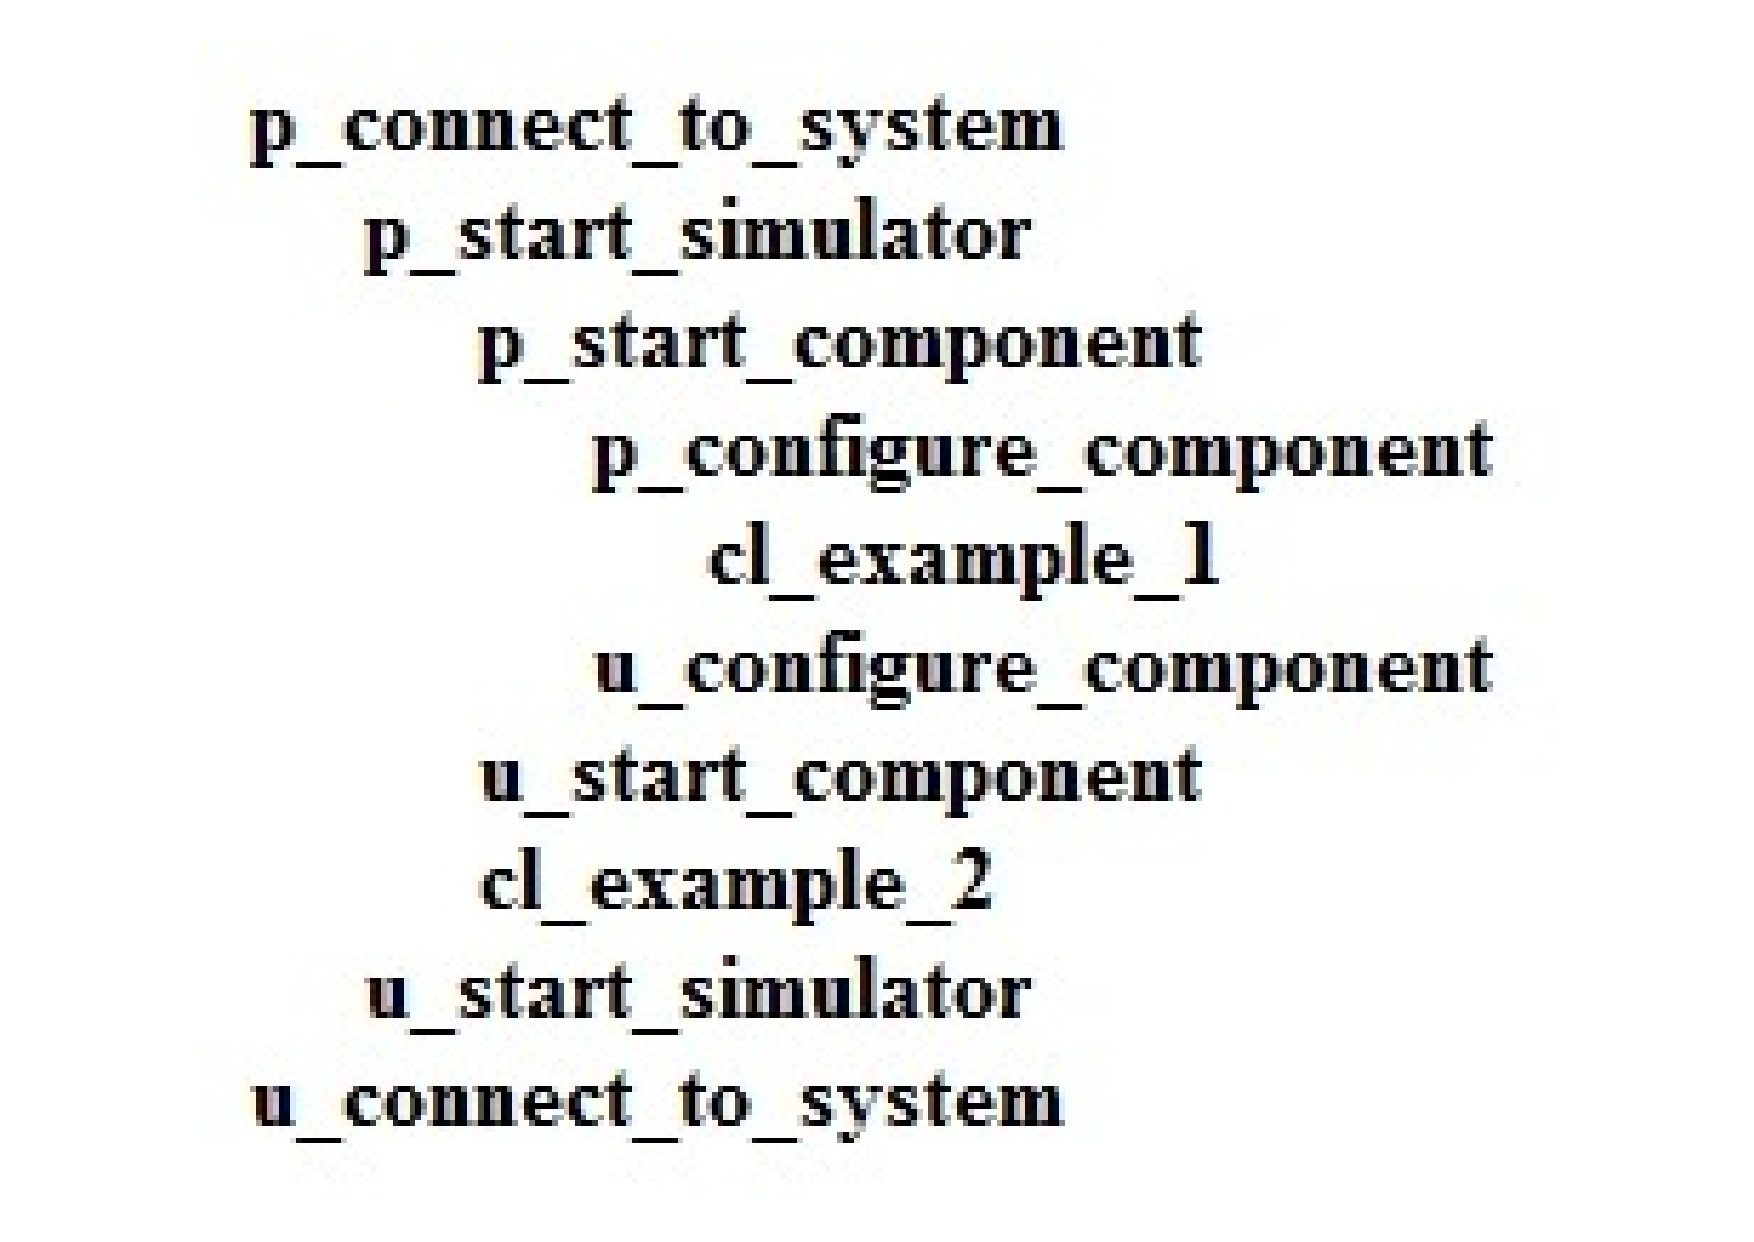
\includegraphics[scale=0.25]{ukazka_planu}
    \caption{Ukážka plánu testov}
    \label{obrazok:ukazka_planu_testov}
    \end{center}
\end{figure}

Jednotlivé testy sa potom vykonávajú sekvenčne. Výhodou tohoto prístupu je, že v~prípade, že sa zmena konfigurácie nepodarila,
daný cluster môžeme preskočiť, a~tým ušetriť čas na dokončenie testovania. 
Test je úspešný, pokiaľ skončí s~nulovou návratovou hodnotou. V~opačnom prípade je test neúspešný. 
Ďalšou výhodou je znovupoužiteľnosť prerekvizít. 
Jednotlivé prerekvizity totiž môžeme kombinovať a~využiť ich tak pre potreby rôznych typov scenárov pre testy. 

Na obrázku \ref{obrazok:ukazka_planu_testov} je znázornený príklad dvoch clusterov, pričom každý z~nich vyžaduje iné nastavenie systému. 
Z~obrázku je vidno, že pre potreby clusteru \texttt {cl\_example\_1} je nutné vykonať prerekvizity \texttt{p\_connect\_to\_system}, 
\texttt{p\_start\_component}, \texttt{p\_start\_simulator} a~prerekvizitu \texttt{p\_configure\_component},
pričom clusteru \texttt{cl\_example\_2} stačia iba dve prerekvizity \texttt{p\_connect\_to\_system} a~\texttt{p\_start\_simulator}.
Nakoľko cluster \texttt{cl\_example\_2} sa spúšťa až za clusterom \texttt{cl\_example\_1}, je nutné vrátiť zmeny systému, ktoré vykonali prerekvizity 
\texttt{p\_start\_component} a~\texttt{p\_configure\_component} pomocou odrekvizít \texttt{u\_start\_component} a~\texttt{u\_configure\_component}.
Jednotlivé prerekvizity na seba môžu, ale nemusia byť závislé, a~preto sa poradie spúšťania prerekvizít môže pre clustre meniť.
Príkladom závislosti môžu byť 2 prerekvizity, kde jedna prerekvizita zapína nejakú súčasť systému s~jeho defaultnými nastaveniami a~druhá prerekvizita 
tieto nastavenia mení. V~druhej prerekvizite môže byť preto nastavené, aby sa spustila, iba ak sa predtým úspešne splnila prerekvizita na zapnutie 
spomínanej časti systému.
Plánovačka testov sa snaží plánovať jednotlivé clustre za seba tak, aby sa nemuseli nutne vykonať všetky prerekvizity a~odrekvizity pre každý cluster zvlášť.
Znamená to, že ak majú dva clustre niektoré prerekvizity rovnaké, tak sa tieto clustre naplánujú tak, že sa rovnaké prerekvizity združia a~spúšťajú sa spravidla len raz. 
Táto vlastnosť je znázornená na obrázku \ref{obrazok:so_zdruzovanim_testov}. Obrázok \ref{obrazok:bez_zdruzovania_testov} znázorňuje plán testov,
ktorý by vznikol ak by plánovač touto vlastnosťou nedisponoval.

\begin{minipage}{\textwidth}
\begin{parcolumns}{2}
\colchunk{\begin{lstlisting}[caption=bez vlastnosti združovania testov,frame=tlrb,label=obrazok:bez_zdruzovania_testov]
p_login  
    cl_test_1
u_login 
p_login 
    p_start_component
        cl_test_2
    u_start_component
u_login
p_login
    p_start_component
        p_configure_component
            cl_test_3
        u_configure_component
    u_start_component
u_login
\end{lstlisting}}

\colchunk{\begin{lstlisting}[caption=s vlastnosťou združovania testov,frame=tlrb,label=obrazok:so_zdruzovanim_testov]






p_login
    cl_test_1
        p_start_component
            cl_test_2
            p_configure_component
                cl_test_3
            u_configure_component
        u_start_component
u_login
\end{lstlisting}}
\colplacechunks
\end{parcolumns}
\end{minipage}

V~regresnej sade sa bežne nachádzajú clustre, ktoré majú rovnakú množinu prerekvizít. Takéto clustre sa radia za seba, aby sa minimalizovalo
spúšťanie prerekvizít a~odrekvizít, ktoré majú spoločné. Neplatí teda pravidlo, že každý cluster má svoju vlastnú unikátnu prerekvizitu.
Tabuľka \ref{tabulka:pocet_testov} zobrazuje prehľad testov v~regresnej sade dvoch najväčších produktoch,
ktoré sa vo firme Acision testujú.

\begin{table}
  \begin{center}
    \begin{tabular}{| c | r | r |}
    \hline
    typ testu & počet testov v~produkte MCO & počet testov v~produkte SMSCv5 \\ \hline
    cluster & 1811 & 1723 \\ \hline
    prerekvizita & 339 & 244 \\ \hline
    odrekvizita & 339 & 244 \\
    \hline
    \end{tabular}
    \label{tabulka:pocet_testov}
    \caption{Prehľad počtu testov v~dvoch najväčších produktoch firmy Acision}
  \end{center}
\end{table}


Medzi ďalšie výhody tohto plánovača testov patrí možnosť špecifikovania pravidiel, s~akými sa budú dané testy spúšťať.
Je napríklad možné nastaviť clusteru zoznam clusterov, takzvaných preoptov, ktoré musia byť úspešne vykonané ešte predtým, ako sa vykoná samotný
cluster. V~prípade, že sa aspoň jeden z~týchto preoptov nevykoná úspešne, cluster sa preskočí.
Výhoda tohto prístupu je v~tom, že ak zo sady testov, ktoré testujú podobnú funkcionalitu, neprejde najzákladnejší test,
môžeme predpokladať, že všetky pokročilejšie testy by neprešli tiež, a~preto ich môžeme preskočiť.

Jednotlivé testy môžeme označovať vhodne zvoleným názvom nejakej funkcionality, pričom môžeme využiť vlastnosť 
plánovača, ktorý nám naplánuje len testy zvolené týmto názvom. Týmto spôsobom môžeme v~regresnej sade vytvárať isté logické celky,
ktoré v~prípade potreby môžeme otestovať samostatne. Pre regresný beh je použitá funkcionalita {\it all}, ktorá združuje 
všetky testy, ktoré nie sú explicitne označené funkcionalitou {\it notall}. Obrázok \ref{obrazok:priklad_spustania_testov} znázorňuje príkaz pre spúšťanie
regresných testov pomocou plánovača testov v~produkte MCO.

\begin{figure}[h]
\begin{lstlisting}
meszarosf@mco-v156#./Run_test.tcl -i cfg.ini -B TEST.REVIEW_23 -f all -wf long_running notall -tw
\end{lstlisting}
\caption{Príklad spúšťania regresných testov pomocou použitého plánovača}
\label{obrazok:priklad_spustania_testov}
\end{figure}

Za zmienku patrí aj možnosť označiť niektoré testy do kategórie označenej ako \textbf{known bugs}.
Testy z~tejto kategórie sú v~prípade zlyhania vylúčené zo zoznamu testov, ktoré zlyhali.
Typicky sa takto označujú testy, ktoré úspešne testujú nejakú funkcionalitu, ale vďaka nejakej nesúvisiacej chybe 
dopadajú neúspechom. Ďalej sa táto funkcionalita využíva napríklad pre testy, ktoré testujú nejakú časť systému,
ktorá sa nestihla do danej vydanej verzie produktu opraviť. V~prípade, ak je test hotový, tak sa nechá v~regresnej sade,
ale pre danú verziu sa označí do kategórie známych chýb, alebo anglicky known bugs.
Takýmto testom je možné explicitne uviesť rozsah verzie softvéru, v~ktorom je tento test chybný.
Tieto testy aj s~verziami softvéru, v~ktorom sa chyby prejavujú, sú uložené v~súbore \textbf{KNOWN.BUGS}.
Príklad označenia testu, ktorý končí neúspechom vďaka nejakej nesúvisiacej chybe je znázornený na obrázku \ref{obrazok:known_bug}.
Tento test testuje chybu, ktorá sa objavila vo verzii produktu 2.3-05.01, avšak opravená bola až vo verzií 2.3-05.02. 

\begin{figure}[h]
\begin{lstlisting}[mathescape]
# MCRD0112570 (Problem with response to SMPP Bind operation)
cl_smpp_028                   >=2.3-05.01 $\sim$ >=2.3-05.02
\end{lstlisting}
\caption{Príklad testu ktorý končí neúspechom pre verziu softvéru 2.3-05.01.}
\label{obrazok:known_bug}
\end{figure}

Spomínaný plánovač testov má ešte veľa vlastností, ktoré už nebudú v~tejto kapitole uvedené, nakoľko predmetom tejto
kapitoly je len jeho stručný popis. Medzi poslednú vlastnosť, ktorú si spomenieme, je možnosť interaktívneho módu.
Interaktívny mód je vlastnosť, ktorá nám umožňuje pozastaviť beh testovania pred alebo za nejakým testom.
Umožňuje prípadne pozastaviť beh testovania ak sa niektorý test ukončí neúspechom. Pozastavenie plánovača znamená,
že je možné si v~špeciálnom režime spúštať vlastné funkcie, alebo celé testy.
Interaktívny mód umožňuje zmeniť beh testovania, na základe špecifických požiadavkov testera, ktorý túto vlastnosť využíva.
Tento mód sa však v~regresných testoch nepoužíva, nakoľko sa narušuje vlastnosť nezávislosti testera na priebehu regresného testovania.

Každý test má svoj zdrojový kód v~spomínanom jazyku TCL a~svoju vlastnú hlavičku, ktorá obsahuje informácie potrebné pre identifikovanie testu a~jeho úspešné zaradenie do regresnej sady.
Zdrojové kódy testov sú logicky rozdelené a~umiestnené v~súboroch začínajúcich predponou {\it CL-} a~s~príponou {\it .tcl}, napríklad {\it CL-SMPP.tcl} alebo {\it CL-GSM.tcl}.
Hlavičky testov môžu byť taktiež logicky delené na niekoľko celkov a~začínajú predponou {\it TEST.}, napríklad {\it TEST.ALL} alebo {\it TEST.REVIEW\_23}.
Takýmto spôsobom sú napríklad delené testy, ktoré prešli kontrolou a~sú úspešne zaradené do regresnej sady (súbor {\it TEST.ALL}) a~testy, ktoré sú do regresnej sady zaradené, ale
zatiaľ neboli nikým skontrolované (súbor {\it TEST.REVIEW\_23}).

Hlavička každého testu je štandardizovaná a~obsahuje nasledovné informácie:
\begin{itemize}
\item \textbf{Name} -- názov testu
\item \textbf{Author} -- autor testu
\item \textbf{Description} -- stručný popis toho, čo daný test vykonáva
\item \textbf{Function} -- názov funkcie v~jazyku TCL, ktorá sa daným testom spustí. Každý test je tvorený jednou funkciou, ktorá je typicky rovnaká
ako názov testu. Ako nepovinný parameter je možné špecifikovať argumenty funkcie. Príkladom môže byť cluster s~názvom \texttt{cl\_send\_sms} ktorý používa
ako argument počet sms správ ktoré má poslať, s~defaultnou hodnotou 100 sms správ.  
má označenú túto položku ako \texttt{cl\_send\_sms 10000}. V~regresnej sade potom existuje test \texttt{cl\_send\_sms\_long\_running}, 
s~položkou Function označenou ako \texttt{cl\_send\_sms 10000}, ktorý posiela takýchto správ stonásobne viac.
\item \textbf{Pre} -- množina všetkých prerekvizít, ktoré musia byť v~čase spustenia daného testu úspešne aktivované. Princíp plánovača je ten,
že prerekvizity sú určené na zmenu stavu testovacieho prostredia. Množina prerekvizít uvedených v~tejto položke teda predstavuje prerekvizity, ktoré
je nutné úspešne spustiť, aby sme testovacie prostredie dostali do stavu, v~ktorom bude možné spustiť aktuálny test.
\item \textbf{Preopt} -- množina všetkých clusterov, ktoré musia byť úspešne spustené v~čase, keď sa púšťa aktuálny test. Ak aspoň jeden cluster z~tejto množiny
dopadol neúspechom, aktuálny cluster sa preskočí. Táto položka je určená iba pre clustre.
\item \textbf{Restore} -- názov prerekvizity, ktorá patrí je určená pre nastavenie testovacieho prostredia pre potreby testu. Táto položka je určená iba pre odrekvizity.
\item \textbf{Undo} -- názov odrekvizity, ktorá je určená pre obnovu testovacieho prostredia. Táto položka je určená iba pre prerekvizity. 
\item \textbf{Functionalities} -- množina všetkých názvov funkcionalít, ktorými je možné daný test spustiť. 
Táto položka umožňuje logicky rozdeliť všetky testy do podmnožín, ktoré je možné spúšťať samostatne. 
Plánovač umožňuje pomocou prepínača \texttt{-f} určiť, ktoré funkcionality sa pri testovaní spustia.
Pred naplánovaním testov sa nájdu sa všetky testy, ktoré sú týmito funkcionalitami označené, a~tieto testy sa naplánujú.
Štandardná hodnota pre všetky clustre je hodnota \texttt{all}, a~pre všetky prerekvizity a~odrekvizity je to hodnota \texttt{notall}.
Typickým príkladom použitia je nastavenie testov, ktoré sa v~nočných regresiách bežne nepúšťajú, 
nakoľko je ich beh príliš časovo náročný, na hodnotu \texttt{long\_running}.
V~plánovači je potom možné spustiť funkcionalitu \texttt{all} bez testov, ktoré sú označené funkcionalitou \texttt{long\_running}.
\item \textbf{Sets} -- umožňuje ďalší spôsob logického rozdeľovania testov na podmnožiny, podobne ako položka \texttt{Functionalities}.
\item \textbf{Versions} -- dolné a~prípadne aj horné ohraničenie hodnoty verzie softwaru, na ktorej je daný test možné pustiť
(Napríklad test určený pre software od verzie 2.3-0.0 vrátane, až do verzie 2.3-04.06 môžeme označiť ako: \textgreater= 2.3-00.00 $\sim$ \textgreater= 2.3-04.06).
\item \textbf{CR} -- popisok slúžiaci na označenie čísla ticketu, alebo čísla zmeny požiadavkov systému\footnote{angl. change request}, ktoré sú do systému implementované
na vyžiadanie zákazníka. 
Pomocou prepínača \texttt{-cr} v~plánovači je možné spustiť všetky testy, ktoré majú dané označenie v~tejto položke.
\item \textbf{CRS} -- informačný popisok slúžiaci na označenie konkrétnej časti naimplementovanej zmeny systému. 
\end{itemize}


Táto sekcia obsahovala zhrnutie toho, akým princípom funguje plánovač testov vytvorený firmou Acision.
Niektoré vlastnosti a~funkcionalita plánovača v~tejto kapitole nie sú popísané, nakoľko nie sú predmetom tejto bakalárskej práce. 
Na záver si ešte uvedieme zoznam výhod a~nevýhod použitia tohoto nástroja.

\noindent \textbf{Výhody}:
\begin{itemize}
\item jednoduché zaradenie nového testu do regresnej sady
\item možná znovupoužiteľnosť prerekvizít
\item združovanie prerekvizít
\item preskakovanie testov o~ktorých vieme, že by skončili neúspechom
\item možné označovanie testov do kategórie známych bugov (súbor KNOWN.BUGS)
\item interaktívny mód pre testovanie
\item označovanie testov do logických celkov a~ich spúšťanie
\item oddelený kód pre zmenu konfigurácie a~pre samotné testy
\item veľká možnosť zmien chovania pomocou prepínačov
\end{itemize} 

\noindent \textbf{Nevýhody}:
\begin{itemize}
\item náhodný neúspech nejakej prerekvizity môže znamenať vynechanie väčšiny testov v~regresnom testovaní
\item jeden chybne pridaný test môže znefunkčniť plánovač
\item jednotlivé testy sa v~prípade chyby systému nemusia úspešne z~tejto chyby zotaviť, a~môžu spustiť lavínu chýb ktoré by inak nenastali 
\item v~prípade, že sa konfiguračné zmeny v~odrekvizitách úspešne neobnovia, dochádzame k~neodpovedajúcim výsledkom z~testovania
\item plánovanie testov je relatívne pomalé
\item prehľad v~testoch a~ich údržba je náročná
\end{itemize}


%
% Kapitola 3
%
\chapter{Návrh riešenia}
\label{kapitola:navrh_riesenia}
Táto kapitola sa zaoberá základným návrhom implementácie rozšírenia plánovača testov pre podporu 
distribuovania testov na viaceré systémy. Kapitola \ref{sekcia:moznosti_distribuovania} popisuje rôzne
možnosti rozdeľovania testov a~ich porovnanie. V~kapitole \ref{sekcia:centralizovana_sprava}
si popíšeme návrh spúšťania testov a~prístup k~centralizovanej správe plánovača testov.
Ďalej kapitola \ref{sekcia:komunikacia} popisuje návrh riešenia komunikácie medzi jednotlivými
regresnými behmi vykonávaných na samostatných testovacích strojoch. V~predposlednej kapitole 
\ref{sekcia:interpretacia_vysledkov} je popísaný návrh zbierania výsledkov a~ich interpretácia.
Posledná kapitola \ref{sekcia:riesenie_novych_problemov} poukazuje na nové typy problémov,
ktoré rozšírením vznikli a~na návrh ich riešenia.



\section{Možnosti distribuovania testov}
\label{sekcia:moznosti_distribuovania}
Pri návrhu distribuovania testov som vychádzal z~informácií o~počte testov a~prerekvizít produktov,
ktoré daný plánovač testov používajú. Informácie som čerpal z~dvoch najväčších produktov (MCO a~SMSCv5), 
ktoré tento plánovač každodenne používajú. Pri každom regresnom behu, sa zbierajú štatistiky o~tom,
koľko testov bolo spustených, a~ako dlho každý test trval. 
V~tabuľkách \ref{tabulka:testy_mco} a~\ref{tabulka:testy_smscv5} sú zobrazené informácie o~testoch z~týchto dvoch najväčších produktov.

\begin{table}
  \begin{center}
    \begin{tabular}{| c | r | r | r | r | r | r |}
    \hline
    typ testu & počet testov & min. čas [s] & max. čas [s] & priem. čas [s] & modus & medián \\ \hline
    cluster      & 1811 & 1 & 931 & 18,47 & 8  & 7 \\ \hline
    prerekvizita & 339  & 1 & 82  & 19,54 & 18 & 1 \\ \hline
    odrekvizita  & 339  & 1 & 63  & 19,56 & 18 & 7 \\
    \hline
    \end{tabular}
    \label{tabulka:testy_mco}
    \caption{Prehľad celkového počtu testov v~produkte MCO}
  \end{center}
\end{table}

\begin{table}
  \begin{center}
    \begin{tabular}{| c | r | r | r | r | r | r |}
    \hline
    typ testu & počet testov & min. čas [s] & max. čas [s] & priem. čas [s] & modus & medián \\ \hline
    cluster      & 1723 & 1 & 1963 & 26,19 & 12 & 3 \\ \hline
    prerekvizita & 224  & 1 & 120  & 9,82  & 6  & 1 \\ \hline
    odrekvizita  & 224  & 1 & 78   & 6,96  & 5  & 1 \\
    \hline
    \end{tabular}
    \label{tabulka:testy_smscv5}
    \caption{Prehľad celkového počtu testov v~produkte SMSCv5}
  \end{center}
\end{table}

Z~tabuliek je vidieť, že produkt MCO má priemerné časy clusterov, prerekvizít a~odrekvizíť veľmi podobné.
V~produkte SMSCv5 je priemerný čas vykonávania clusterov niekoľkonásobne vyšší, ako priemerný čas vykonávania prerekvizít alebo odrekvizít.
Tieto tabuľky však ukazujú celkový počet všetkých testov. Niektoré testy sa však sú však z~regresnej sady vynechané.
Navyše z~tabuliek nie je jasné, koľko prerekvizít sa skutočne naplánuje pre jeden beh regresií.
Z~konceptu plánovača totiž vyplýva, že niektoré prerekvizity je nutné púšťať viacnásobne.
Je to preto, lebo každý cluster môže mať inú množinu prerekvizít, a~všetky tieto kombinácie možných prerekvizít pre každý cluster
je potrebné naplánovať.

\begin{table}
  \begin{center}
    \begin{tabular}{| c | r | r |}
    \hline
    typ testu  & počet testov pre produkt MCO & počet testov pre produkt SMSCv5 \\ \hline
    cluster      & 1702 & 1650 \\ \hline
    prerekvizita & 706  & 596  \\ \hline
    odrekvizita  & 706  & 596 \\
    \hline
    \end{tabular}
    \label{tabulka:pocet_naplanovanych_testov}
    \caption{Prehľad počtu naplánovaných testov pri spúšťaní regresií v~produktoch MCO a~SMSCv5}
  \end{center}
\end{table}

Tabuľka \ref{tabulka:pocet_naplanovanych_testov} zobrazuje počet clusterov a~prerekvizít, ktoré sa plánujú
pri každodennom spúšťaní nočných regresií pomocou funkcionality \texttt{all}. Z~tabuľky vyplýva, že približne 5\% testov sa 
z~nočných regresií vynecháva. Túto množinu tvoria napríklad testy, ktoré nie sú plne automatické, a~vyžadujú tak interakciu s~používateľom,
alebo testy o~ktorých sa vie, že je nevhodné ich púšťať spolu s~veľkou množinou testov.
Zároveň z~obrázku vypláva to, že sa spustí viac ako dvojnásobok prerekvizít, ako existuje v~testovacej sade.
Každá prerekvizita sa teda spustí v~priemere viac ako dvakrát. 
Vo svetle týchto informácií je teda vhodné zameriavať sa pri rozdeľovaní testov na clustre.

V~nasledujúcej časti sa pozrieme na navrhnuté možnosti distribuovania testov, ich výhody a~nevýhody.
Treba podotknúť, že plánovač testov si uchováva čas behu každého naposledy spusteného testu.
Táto štatistika sa môže využiť pri distribuovaní testov, aby sme vedeli rovnomerne rozložiť záťaž pre každý systém.
\subsubsection*{Distribúcia clusterov na základe času behu clusteru}
Tento princíp distribúcie by spočíval v~rozdeľovaní clusterov do n podmnožín na základe súčtu časov, 
trvaní všetkých clusterov, v~danej podmnožine. Každý cluster by bol zaradený do jednej podmnožiny, pričom by platilo,
že každá podmnožina by sa spúšťala na samostatnom testovacom systéme. Pri rozdeľovaní testov na podmnožiny by sa bral zreteľ na
distribuovanie záťaže.

\noindent \textbf{Výhody}:
\begin{itemize}
\item jednoduché na implementáciu
\end{itemize} 

\noindent \textbf{Nevýhody}:
\begin{itemize}
\item odhadovaný čas každej podmnožiny clusterov by nereflektoval stav po naplánovaní, pretože by
neobsahoval čas potrebný pre spustenie prerekvizít a~odrekvizít
\item neefektívne združovanie prerekvizít
\item nerovnomerné rozloženie záťaže
\end{itemize}

\subsubsection*{Distribúcia clusterov na základe spoločných prerekvizít}
Distribúcia na základe spoločných prerekvizít využíva faktu, že v~regresnej sade existujú testy, ktoré majú rovnakú množinu prerekvizít.
Celú regresnú sadu môžeme týmto spôsobom rozdeliť na \emph{n} podmnožín, pričom by platilo, že všetky clustre v~jednej takejto množine by mali
rovnakú množinu prerekvizít. Pri distribúcií testov na \emph{m} častí, ktoré by sa spúšťali samostatne, by sa do jednotlivých \emph{m} častí
priraďovali vždy celé podmnožiny \emph{n}. Obrázok \ref{obrazok:podmnoziny_testov} ilustruje delenie clusterov do štyroch \emph{n} podmnožín.
Pri distribúcií testov by sa potom každá takáto podmnožina brala ako celok, a~distribuovali by sme tak jednotlivé podmnožiny.
Obrovskou výhodou tohoto prístupu je to, že vo výsledku by sme ušetrili spúšťanie niekoľkých prerekvizít, nakoľko by sa
využila vlastnosť plánovača, a~tou je združovanie testov. Príkladom výsledku môže byť napríklad distribuovanie testov na 2 systémy, 
pričom prvý systém by spúšťal clustre z~podmnožiny 1 a~4 (clustre \texttt{cl\_podmnozina1\_test1}, \texttt{cl\_podmnozina1\_test2} a~\texttt{cl\_podmnozina4\_test1})
a~druhý systém by spúšťal clustre z~podmnožiny 2 a~3 (clustre \texttt{cl\_podmnozina2\_test1}, \texttt{cl\_podmnozina2\_test2}, 
\texttt{cl\_podmnozina2\_test3}, \texttt{cl\_podmnozina3\_test1} a~cluster \texttt{cl\_podmnozina3\_test2}).


\begin{figure}[h]
\begin{lstlisting}
p_login
    cl_podmnozina1_test1
        p_start_component
            cl_podmnozina2_test1
            cl_podmnozina2_test2
            cl_podmnozina2_test3
            p_configure_component
                cl_podmnozina3_test1
                cl_podmnozina3_test2
            u_configure_component
        u_start_component
    cl_podmnozina1_test2
    p_start_simulator
        cl_podmnozina4_test1
    u_start_simulator
u_login
\end{lstlisting}
\caption{Príklad rozdeľovania clusterov na podmnožiny na základe spoločných prerekvizít}
\label{obrazok:podmnoziny_testov}
\end{figure}

\noindent \textbf{Výhody}:
\begin{itemize}
\item náročnejšie na implementáciu
\item lepšie rozloženie záťaže
\item zníženie času potrebného pre dokončenie testovania využitím vlastnosti združovania testov
\end{itemize} 

\noindent \textbf{Nevýhody}:
\begin{itemize}
\item nedokonalé združovanie prerekvizít 
\item odhadovaný čas každej podmnožiny clusterov by nereflektoval stav po naplánovaní, pretože by
neobsahoval čas potrebný pre spustenie prerekvizít a~odrekvizít
\end{itemize}

\subsubsection*{Distribúcia clusterov na základe častí plánu}
Idea tohoto prístupu spočíva v~tom, že by sa všetky testy naplánovali ako obvykle, a~po naplánovaní by sa
celý plán rozdelil na \emph{m} častí. Plánovač by spočítal odhadované časy jednotlivých častí, a~snažil by sa tieto časti
rozdeliť rovnomerne. Po rozdelení by sa do každej časti museli pridať prerekvizity a~odrekvizity, o~ktoré
by sme daným delením prišli. Princíp rozdelenia plánu na 3 časti je znázornený na obrázku \ref{obrazok:distribucia_na_casti}.
\begin{figure}[h]
\begin{lstlisting}
p_login
    cl_test01
    p_start_component
        cl_test02
        cl_test03
        cl_test04
        p_configure_component
            cl_test05
----------------------------------
            cl_test06
        u_configure_component
    u_start_component
    cl_test07
    p_start_simulator
        cl_test08
        cl_test09
----------------------------------
        cl_test10
        cl_test11
        cl_test12
        cl_test13
    u_start_simulator
u_login
\end{lstlisting}
\caption{Príklad rozdeľovania clusterov na základe častí plánu}
\label{obrazok:distribucia_na_casti}
\end{figure}

Po rozdelení je jasné, že každej časti musíme pridať prerekvizity a~odrekvizity
o~ktoré sme prišli pri delení. Ak sa tieto testy pridajú do plánu, celý plán
pre 3 systémy by vyzeral tak, ako je znázornené na obrázku \ref{obrazok:distribucia_casti_po_preplanovani}.
Z~obrázku je jasné, že pre vysoký počet testov by bol tento prístup najvhodnejší.
Problémom tohoto prístupu je však to, že požiadavkom na funkcionalitu plánovača bolo to,
aby sa princíp plánovania testov nezmenil. Znamená to, že by sa museli rešpektovať hlavičky testov
napríklad na položku \emph{Preopt}, čo znamená, že každému clusteru môžeme nastaviť množinu clusterov,
ktoré musia byť úspešne otestované ešte predtým, ako sa spustí test aktuálneho clusteru.
Príkladom tohoto problému je prípad, kedy by cluster cl\_test13 mal nastavený 
\emph{Preopt} na cluster \emph{cl\_test01} a~\emph{cl\_test06}.
V~praxi by to znamenalo, že celá tretia časť rozdeleného plánu by sa musela preplánovať,
a~spomínané clustre by sa do nej museli pridať. Ďalšou nevýhodou je to, že tento prístup by
vyžadoval väčší zásah do funkčnosti plánovača testov, nakoľko by sa celá logika plánovača musela upraviť.
V~prípade, že by ale neexistoval požiadavok na zachovanie funkčnosti, tento prístup by bol najvhodnejší.
Týmto problémom, spôsobeným zachovaním funkcionality plánovača, trpia aj predošlé 2 spôsoby distribúcie testov. 
Pre povahu testov v~regresnej sade by však najviac na toto doplácal práve tento princíp distribuovania testov.  

\noindent \textbf{Výhody}:
\begin{itemize}
\item efektívne združovanie prerekvizít
\item veľmi presné rozloženie záťaže (v~prípade nezachovania požiadavkov na funkcionalitu)
\item presný odhad trvania testovania (v~prípade nezachovania požiadavkov na funkcionalitu)
\end{itemize} 

\noindent \textbf{Nevýhody}:
\begin{itemize}
\item náročné na implementáciu, pretože by sa musela zmenila logika plánovača
\end{itemize}

\begin{figure}[h]
\begin{lstlisting}
p_login
    cl_test01
    p_start_component
        cl_test02
        cl_test03
        cl_test04
        p_configure_component
            cl_test05
        u_configure_component
    u_start_component
u_login

p_login
    p_start_component
        p_configure_component
            cl_test06
        u_configure_component
    u_start_component
    cl_test07
    p_start_simulator
        cl_test08
        cl_test09
    u_start_simulator
u_login

p_login
    p_start_simulator
        cl_test10
        cl_test11
        cl_test12
        cl_test13
    u_start_simulator
u_login
\end{lstlisting}
\caption{Príklad rozdeľovania clusterov na základe častí plánu - po preplánovaní}
\label{obrazok:distribucia_casti_po_preplanovani}
\end{figure}
 

\section{Centralizovaná správa plánovača}
\label{sekcia:centralizovana_sprava}
Jedným z~hlavných vlastností, spomínaných v~dokumente \cite{Parallel_approach}, ktoré by mal mať nástroj pre distribúciu testov,
je vlastnosť centralizovanej správy všetkých testov. 
Pri návrhu rozšírenia plánovača sa táto vlastnosť brala v~úvahu. 
Rozšírenie je navrhnuté tak, aby bolo z~jedného stroja spustiť rozšírený plánovač, ktorý by rozdelil množinu testov na \emph{m} 
podmnožín, v~závislosti na počtu strojov, na ktorých chceme regresné testy spustiť. Jednotlivé podmnožiny testov sa 
potom predajú novým inštanciám plánovačom testov, ktoré by tieto testy preplánovali a~začali by ich vykonávať. 
Tieto nové inštancie plánovačov sú spustené ako podprocesy hlavného procesu, ktorým je rozšírený plánovač testov.
Plánovač testov je navrhnutý tak, aby dokázal rozdistribuovať testy na teoreticky nekonečný počet neprázdnych podmnožín.
V~prípade, že je počet testovacích systémov väčší ako počet clusterov, niektoré testovacie systémy sa nevyužijú.
Centralizovaná správa plánovača umožňuje zobraziť rozdelený plán testovania pre každý testovací systém zvlášť.
Zároveň umožňuje vypísať odhadované časy testovania pre každý systém zvlášť a~umožňuje porovnanie efektivity distribuovania testov voči stavu,
kedy by testy neboli distribuované a~spúšťali by sa iba na jednom systéme. 

Pri navrhovaní riešenia pre centralizovanú správu testov, bolo nutné vymyslieť akou formou sa budú spúšťať 
jednotlivé inštancie plánovača pre distribuované systémy. Plánovač testov totiž potrebuje konfiguračný súbor,
zadávaný parametrom \textbf{-i}, ktorý je uvedený napríklad na obrázku \ref{obrazok:priklad_spustania_testov}..
Tento konfiguračný súbor informácie ako IP adresa systému, na ktorom sa budú spúšťať testy, číslo verzie softvéru, názov 
produktu, atď. Príklad takéhoto konfiguračného súboru je znázornený na obrázku \ref{obrazok:priklad_konfig_suboru}.
Rozšírenie plánovača pre distribuované systémy však potrebuje informácií obsiahnutých v~konfiguračnom súbore viac.
Pre každý distribuovaný systém potrebuje napríklad jednu IP adresu obsiahnutú v~položke \textit{Host}.
Jedným riešením by bolo dať všetky informácie pre každý distribuovaný systém do jedného konfiguračného súboru.
V~tomto jednom súbore by sa potom dalo napríklad nastavovať, na koľkých testovacích systémoch sa regresné testy spustia.
Pre toto riešenie by však trebalo upraviť parser, ktorý informácie z~týchto konfiguračných súborov vyhodnocuje.
Mnou navrhnuté riešenie teda počíta s~jedným konfiguračným súborom pre každý testovací systém.
Pri spúšťaní regresných testov na troch systémoch, je preto potrebné mať pripravené 3 konfiguračné súbory,
každý pre jeden testovací systém. 

\begin{figure}[h]
\begin{lstlisting}
Product: MCO
Username: root
Host: 10.10.10.206
Outerhost: 10.10.110.206
Version: 2.3-05.04
\end{lstlisting}
\caption{Príklad konfiguračného súboru pre produkt MCO}
\label{obrazok:priklad_konfig_suboru}
\end{figure}

Nová funkcionalita, ktorá bola pridaná do rozšíreného plánovača je možnosť sledovať aktuálny stav testovania
formou progress baru. Táto funkcionalita v~starej verzií plánovača testov chýbala, a~bolo pre to ťažké sledovať aktuálny
stav testovania. V~rozšírenej verzií plánovača sa zobrazuje aktuálny stav testovania pre každý systém zvlášť, ako aj
celkový stav všetkých testov.

\section{Komunikácia medzi jednotlivými plánovačmi testov}
\label{sekcia:komunikacia}
V~distribuovaných systémoch nie je spoločná pamäť, a~preto je forma komunikácie založená na princípe zasielania správ.
Princíp komunikácie je taký, že hlavný proces, ktorý spustí \emph{m} plánovačov testov vo forme podrocesov, čaká na ukončenie
všetkých týchto podprocesov. Ukončenie podprocesu znamená, že ak nenastala žiadna systémová chyba, tak je testovanie jednej
podmnožiny testov dokončené. Ak by náhodou nastala nejaká kritická chyba, podproces by sa mohol ukončiť, a~my by sme mohli prísť
o~výsledky z~tejto podmnožiny regresných testov. Z~tohoto dôvodu by sa výsledky z~testovania mali posielať ihneď, ako ich máme k~dispozícií,
a~nemalo by sa čakať na dokončenie testovania danej podmnožiny regresných testov. Každý podproces teda asynchrónne zasiela údaje o~výsledkoch
aktuálneho testu hlavnému procesu, ktorý si tieto výsledky uchováva. Tento prístup má výhodu, že sa výsledky testovania uchovávajú na dvoch miestach,
a~v~prípade zlyhania systému, či už hlavného procesu alebo podprocesov, by sme sa k~daným výsledkom vedeli dopracovať. 


\section{Interpretácia výsledkov}
\label{sekcia:interpretacia_vysledkov}
Medzi jednu z~najdôležitejsích vlastností, ktoré musí každý testovací nástroj mať, je vlastnosť zobrazovania výsledkov z~testovania.
Pri návrhu rozšírenia plánovača testov bolo nutné riešiť situáciu, ako zobraziť výsledky z~každého testovacieho systému jednotlivo,
a~takisto aj súhrn celkových výsledkov. 

Rozšírenie plánovača testov disponuje niekoľkými výsledkami, ktorými môže každý test skončiť. 
Jednotlivé výsledky platia len v~prípade, že sa daný test spúšťal na všetkých testovacích systémoch len raz. Sú to výsledky:
\begin{itemize}
\item \textbf{passed} -- test ktorý sa skončil úspechom (návratová hodnota je rovná nule).
\item \textbf{failed} -- test ktorý sa ukončil neúspechom (nenulová návratová hodnota).
\item \textbf{skipped} -- test ktorý sa vďaka neúspechu nejakého predošlého testu vynechal, nakoľko by jeho spustenie skončilo neúspechom.
\item \textbf{passed on second attempt} -- cluster ktorý sa vďaka prepínaču plánovača \textbf{-tw} spustil po neúspechu znova, pričom na druhý
krát skončil úspechom. Test označený týmto výsledkom je zároveň označený výsledkom \textbf{passed}
\item \textbf{known bug - failed} -- cluster ktorý je pre aktuálnu verziu softvéru označený ako \textbf{known bug}, ktorý skončil úspechom. 
Cluster označený týmto výsledkom nie je označený výsledkom \textbf{failed}.
\item \textbf{known bug - passed} -- cluster ktorý je pre aktuálnu verziu softvéru označený ako \textbf{known bug}, ktorý skončil neúspechom.
Cluster označený týmto výsledkom je zároveň označený aj výsledkom \textbf{passed}.
\end{itemize} 

V~prípade, že sa nejaký test spúšťal na viacerých systémoch, bolo nutné riešit stav, v~ktorom sa test mohol ocitnúť. 
Problémom je situácia, kedy nejaký test, ktorý sa spúšťal na viacerých systémoch, skončil na týchto rozdielnych systémoch rôznymi výsledkami.
Pre riešenie tejto situácie bol zavedený stav \textbf{unclear}. 
Ak test skončí s~rôznymi výsledkami, jeho finálny výsledok sa určí podľa prevodovej tabuľky \ref{tabulka:vysledky_testu_prevod}.
Stavy \emph{passed on second attempt}, \emph{known bug - failed}
a~\emph{known bug - passed} nie sú zaznačené z~dôvodu, že tieto špeciálne stavy sa mapujú na stavy \emph{failed} a~\emph{failed}.

Spomínané stavy výsledkov testov platia pre celkové výsledky zo všetkých testovacích systémov. Rozšírený plánovač testov navyše umožňuje zobraziť 
výsledky všetkých testov pre každý testovací systém jednotlivo. Výsledok každého testu sa zobrazuje v~rovnakom poradí, ako sa testy spúšťali.
Každý zobrazovaní výsledkov z~každého testovacieho systému majú však testy pre jednoduchosť len stavy \emph{passed}, \emph{failed} a~\emph{skipped}. 

\begin{table}
  \begin{center}
    \begin{tabular}{| c | c | c |}
    \hline
    výsledok 1  & výsledok 2 & konečný výsledok \\ \hline
    passed      & passed     & passed  \\ \hline
    failed      & failed     & failed  \\ \hline
    skipped     & skipped    & skipped \\ \hline
    passed      & skipped    & passed  \\ \hline
    failed      & skipped    & failed  \\ \hline
    passed      & failed     & unclear \\ \hline
    unclear     &      *     & unclear \\ 
    \hline
    \end{tabular}
    \label{tabulka:vysledky_testu_prevod}
    \caption{Mapovanie rozdielnych výsledkov testu na konečný výsledok}
  \end{center}
\end{table}



\section{Riešenie nových typov problémov}
\label{sekcia:riesenie_novych_problemov}
Pri vytváraní rozšírenia plánovača je potrebné myslieť na nové problémy, ktoré sa objavili
až pri riešení distribúcie testov. Jedným z~problémov je zobrazovanie výsledkov testov spomínané v~predchádzajúcej kapitole.
Pre riešenie tohoto problému bol zavedený výsledok testu\emph{unclear}.

\subsection*{Nezávislosť medzi testami}
Ďalším z~problémov, ktorého riešenie bolo treba navrhnúť, bol problém, ktorý porušoval vlastnosť nezávislosti 
medzi testami a~vlastnosť integrity testovacej sady, popísaných v~dokumente \cite{Kapfhammer}.
Jednalo sa o~problém, že niektoré testy používali pevne stanovený sieťový port, ktorý slúžil napríklad pre
komunikáciu so simulátorom, alebo pre napojenie sa na nejakú časť testovaného systému, atď.
Problémom tohoto pevného portu bola distribúcia testov, ktoré používali rovnaký port.
V~prípade, že sa takéto testy spúšťali naraz, dochádzalo k~obsadeniu portu prvým testom, pričom druhý test 
už k~portu nemal prístup, a~tak končil neúspechom.

Riešením tohoto problému je parameter port offset \textbf{-po}. 
Každý test, ktorý používal pevne stanovenú hodnotu portu sa musel upraviť tak, aby 
sa ako port použila táto pevná hodnota pripočítaná o~hodnotu zadanú parametrom \textbf{-po}.
Jednotlivé podprocesy plánovača testov sa spúšťajú s~parametrom \textbf{-po}, ktorý sa
navyšuje práve o~hodnotu \textbf{-po} s~každým podprocesom.
V~praxi to znamená, že ak nastavíme hodnotu offsetu na 1000, tak sa prvý podproces spustí s~parametrom
\textbf{-po 1000}, druhý podproces sa spustí s~parametrom \textbf{-po 2000}, tretí s~\textbf{-po 3000} atď.
V~teste sa potom používa štandardné číslo portu, ktorý sa využíval v~teste pred úpravou, s~pridanou hodnotou port offsetu.
Týmto spôsobom sa zabraňuje problému, že niektoré testy pristupovali k~rovnakému portu súčastne.
Implicitnou hodnotou parametru \textbf{-po}, ktorá sa používa napríklad pri spustení plánovača testov
bez potreby distribúcie testov je hodnota 0. 

\subsection*{Systém logovania}
Ďalším novým problémom sa stalo aj spravovanie logovacích súborov. Plánovač testov totiž
pri vykonávaní testov zapisuje informácie o~aktuálne prevádzaných testoch do viacerých logovacích súborov.
Pri distribuovaní testov sa však spúšťajú viaceré podprocesy plánovača testov, pričom každý podproces
si tieto súbory vytvára zvlášť. V~rámci centrálnej správy bolo nutné navrhnúť prístup, akým sa budú
logovať testy z~viacerých strojov na jedno centrálne miesto.
Pre riešenie tohoto problému bolo možné implementovať 2 možné spôsoby:
\begin{itemize}
\item \textbf{Zapisovanie údajov do logov po každom teste} -- týmto spôsobom by sa do logovacích súborov vytváraných hlavným procesom
postupne zapisovali informácie, vždy po aktuálne dokončenom teste, nezávisle na testovacom systéme.
Tento prístup je však nevyhovujúci, lebo by podprocesy museli posielať logovacie informácie hlavnému procesu, čo je náročné na zdroje.
Ďalšou nevýhodou je to, že by sa poradie jednotlivých testov z~testovacích systémov pomiešalo.
\item \textbf{Parsovanie údajov do logov po dokončení testovania} -- toto riešenie spočíva v~tom, že
sa najprv počká na dokončenie testovania. V~momente, ak je testovanie ukončené, môžeme počítať so situáciou,
že každý podproces plánovačky testov si vytvoril vlastné logovacie súbory, v~ktorých je zachované poradie testov.
Ak máme tieto súbory k~dispozícií, môžeme si z~nich vytiahnuť potrebné informácie a~skopírovať ich do logovacích
súborov vytvorených rozšíreným plánovačom testov. Toto riešenie má výhodu, že je menej náročné na zdroje, a~zároveň
že sa v~logoch dodržiava poradie testov vykonávaných pre každý systém zvlášť. 
Pri implementácií rozšírenia plánovača testov sa využíva práve toto riešenie.
\end{itemize} 



%
% Kapitola 4
%
\chapter{Implementácia}
\label{kapitola:implementacia}
Kapitola popisuje základné implementačné detaily jednotlivých častí rozšírenia pre plánovač testov.
Prvá kapitola popisuje, aké technológie boli pre implementáciu rozšírenia plánovača použité.
Nakoľko sa jedná o~implementáciu rozšírenia pre nástroj, ktorý už bol vytvorený, kapitola taktiež popisuje 
rozdelenie zdrojového kódu na časť vytvorenú firmou Acision, a~časť vytvorenú mnou.
Kapitola \ref{sekcia:distribucia_testov} popisuje implementáciu distribúcie testov so zameraním na 
rozloženie záťaže. Tretia kapitola popisuje, akou formou sa spúšťajú testy na jednotlivých testovacích
systémoch. Táto kapitola ďalej popisuje implementáciu komunikácie medzi jednotlivými procesmi plánovača testov.
Posledná kapitola \ref{sekcia:sledovanie_stavu} popisuje implementáciu novej funkcionality plánovača, ktorou je progress bar.

\section{Použité technológie a~členenie práce}
\label{sekcia:pouzite_technologie}
Rozšírenie plánovača testov je napísané v~jazyku Tcl/Tk (Tool Command Language), pre verziu 8.4.19.
Plánovač testov je vo firme známy pod názvom TTT (Tcl Testing Tool).
Pre každý produkt je delený na 2 časti, pričom každá časť sa udržiava v~samostatnom repozitáry vo verzovacom systéme.
Jedná sa o~časti: 
\begin{itemize}
\item \textbf{ttt-core} -- Je logická časť plánovača testov, zodpovedná predovšetkým za plánovanie, zbieranie výsledkov,
spúšťanie testov, vytváranie logov a~pod. Táto časť je spoločná pre všetky produkty. 
\item \textbf{ttt-product} -- Je časť plánovača testov, ktorá obsahuje všetky testy, simulátory a~nástroje potrebné pre 
otestovanie špecifického produktu. Nakoľko sa plánovač testov využíva pre testovanie širokej škály produktov, 
každý produkt má vlastný repozitár pre svoje testy, ktorý si udržiava oddelene.
\end{itemize} 

Pri vytváraní rozšírenia pre plánovač testov som zasahoval hlavne do časti \textbf{ttt-core}, ktorá je spoločná pre každý produkt.
Táto časť je rozdelená na niekoľko súborov. Pri implementovaní som všetky mnou vytvorené funkcie a~zdrojový kód vkladal do
mnou vytvoreného súboru \textbf{prlmng.tcl}. Tento súbor obsahuje všetky funkcie potrebné pre správnu funkcionalitu rozšírenia.
Pri vytváraní rozšírenia sa však niektoré časti kódu museli upraviť. Jednalo sa hlavne o~hlavný súbor plánovačky testov, súbor
\textbf{Run\_test.tcl} a~o~súbor zodpovedný pre plánovanie testov, súbor \textbf{tstmng.tcl}. 
Zmeny prevedené v~súbore \textbf{Run\_test.tcl}:


Zmeny prevedené v~súbore \textbf{tstmng.tcl}:

Nakoľko firma Acision vyvýja komerčný softvér, pri odovzdávaní zdrojových kódov 
som pre ochranu duševného vlastníctva firmy Acision odovzdal len súbory nutné pre 
beh plánovača testov. Pri odovzdávaní som dodržal logickú štruktúru testov, ktoré sa
v~produkte MCO používajú, avšak zdrojové kódy testov som musel nahradiť jednoduchou funkciou,
ktorá počká náhodný čas a~potom ukončí test úspechom.
Odovzdané súbory obsahujú štatistický súbor \textbf{TTT\_stat.txt}, ktorý uchováva časy vykonávania
každého testu spúšťaného v~regresnej sade produktu MCO. Tento súbor obsahuje presné informácie o~dĺžke
behu testov v~tomto produkte, a~je použitý pre porovnanie výsledkov.
Ďalej je medzi odovzdanými súbormi súbor \textbf{KNOWN.BUGS} z~produktu MCO. Tento súbor obsahuje testy
ohraničené verziami, v~ktorých sa vyskutujú odhalené chyby, ktoré nemusia priamo súvisieť
s~funkcionalitou, ktorá sa v~danom teste testuje. Viac sa o~súbore \textbf{KNOWN.BUGS} píše v~kapitole \ref{sekcia:princip_pouziteho_planovaca}.
Z~časti \textit{ttt-core} som odovzdal len súbory nutné pre beh plánovača. 

\section{Distribúcia testov}
\label{sekcia:distribucia_testov}
Pri implementovaní distribúcie testov som použil distribúciu clusterov na základe spoločných prerekvizít, 
popísanú v~kapitole \ref{sekcia:moznosti_distribuovania}.
Implementácia distribuovania testov je obsiahnutá vo funkcií \texttt{prl\_divide\_test\_groups}.

Táto funkcia sekvenčne prejde všetky testy, a~rozdelí ich do skupín kde každý cluster v~rovnakej skupine,
má rovnakú množinu prerekvizít. Pre každú takúto skupinu sa potom spočíta odhadovaný čas behu tejto skupiny.
Odhadovaný čas sa ráta na základe posledného času behu daného clusteru, zaznamenanom v~súbore \textit{TTT\_stat.txt}.
Tieto skupiny sa potom zoradia podľa odhadovaného času behu celej skupiny.
V~cykle sa potom prechádzajú tieto skupiny od najväčšej po najmenšiu, a~postupne sa priraďujú 
do jedného z~\emph{m} zoznamov spúšťaných clusterov na distribuovaných systémoch.

Vylepšením implementácie tohoto algoritmu sa neskôr venuje kapitola \label{kapitola:optimalizacie}. 


\section{Spúšťanie podprocesov a~komunikácia s~nimi}
\label{sekcia:spustanie_podprocesov}


\section{Sledovanie aktuálneho stavu testovania}
\label{sekcia:sledovanie_stavu}

\section{Zbieranie a~vyhodnocovanie výsledkov}
\label{sekcia:zbieranie_vysledkov}




%
% Kapitola 5
%
\chapter{Optimalizácie rozdeľovania testov}
\label{kapitola:optimalizacie}




%
% Kapitola 6
%
\chapter{Zhodnotenie dosiahnutých výsledkov}
\label{kapitola:zhodnotenie_vysledkov}

\section{Prínos použitia paralelného plánovača testov}
\label{sekcia:prinos_pouzitia}

\section{Porovnanie jednotlivých optimalizácií}
\label{sekcia:porovnanie_optimalizacii}

%
% Kapitola 7
%
\chapter{Záver}
\label{kapitola:zaver}

\section{Zhrnutie}
\label{sekcia:zhrnutie}

\section{Možnosti ďalšieho vývoja}
\label{sekcia:moznosti_dalsieho_vyvoja}
%=========================================================================
